\documentclass[]{article}
%document colors
\usepackage{xcolor}
\definecolor{favoritecolor1}{HTML}{607CB2}
\definecolor{favoritecolor2}{HTML}{303E59}
\makeatletter
\newcommand{\globalcolor}[1]{%
	\color{#1}\global\let\default@color\current@color
}
\makeatother

\AtBeginDocument{\globalcolor{favoritecolor2}}
\pagecolor{favoritecolor1}

%made from template named MathArticleTemplate
\usepackage{amsfonts}
\usepackage{amsmath}
\usepackage{amsthm}
\usepackage{amssymb}
\usepackage{hyperref}
\hypersetup{colorlinks=true}
\usepackage{graphics}
\usepackage{graphicx}

%Fix \eqref in section title
\pdfstringdefDisableCommands{\def\eqref#1{(\ref{#1})}}

\DeclareMathOperator{\arsinh}{arsinh}
\DeclareMathOperator{\arcosh}{arcosh}
\DeclareMathOperator{\artanh}{artanh}
\DeclareMathOperator{\rues}{rues}
\DeclareMathOperator{\md}{mod}
\DeclareMathOperator{\pow}{Pow}
%Parenthesis, Braces, Brackets usepackage{physics}
\newcommand{\pqty}[1]{{\left(#1\right)}}
\newcommand{\Bqty}[1]{{\left\{#1\right\}}}
\newcommand{\bqty}[1]{{\left[#1\right]}}
\newcommand{\abs}[1]{{\left\lvert#1\right\rvert}}
%other stuff
\newcommand{\floor}[1]{{\left\lfloor#1\right\rfloor}}
\newcommand{\ceil}[1]{{\left\lceil#1\right\rceil}}
%Laplace transform and inverse
\newcommand{\laplace}[1]{\mathcal{L}\Bqty{#1}\pqty{s}}
\newcommand{\laplaceInv}[1]{\mathcal{L}^{-1}\Bqty{#1}\pqty{t}}
%Derivatives
\newcommand{\pdiff}[2]{\frac{\partial^{#2}}{\partial #1^{#2}}}

%lemma,theorem, proof
\newtheorem{theorem}{Theorem}[section]
\newtheorem{lemma}[theorem]{Lemma}
\newtheorem{definition}[theorem]{Definition}
\newtheorem{corollary}[theorem]{Corollary}

\numberwithin{equation}{section}

\usepackage{xr}

%\usepackage{minted}
%opening
\author{Mark Andrew Gerads: \href{MailTo:Nazgand@Gmail.Com}{Nazgand@Gmail.Com}}

\title{
	Hyperbolic Plane Metrics
	
	\href{https://github.com/Nazgand/nazgandMathBook}{https://github.com/Nazgand/nazgandMathBook}
}

\begin{document}
	
	\maketitle
	
	\begin{abstract}
		The goal of this paper is to introduce the Polar Hyperbolic Plane Metric and the Cartesian Hyperbolic Plane Metric. These metrics are useful because they both map the entire Euclidean plane to the entire Hyperbolic plane.
	\end{abstract}
	
	\section{Circumference as a Function of Radius and Curvature}
	Let $R=\frac{1}{\sqrt{-K}}$, where $K$ is the Gaussian curvature of the Hyperbolic Plane. Then the circumference of a circle with radius $r$ is
	\begin{equation}
	C\pqty{R,r}=2\pi R\sinh\pqty{\frac{r}{R}}
	\end{equation}
	However, looking ahead, the models we obtain in the general case are essentially scaled versions of the case $K=-1\land R=1$. E.g. distance $d$ in a model where $R\in\mathbb{R}^+$ is isomorphic to distance $\frac{d}{R}$ in a model where $R=1$.
	
	\section{Polar Hyperbolic Plane Metric}
	In this model, we desire the distance from the origin to be $r$, both in [the Euclidean sub-space the model is built on] and in [the Hyperbolic space of the model]. This model requires changing the density of space along the circles surrounding the origin by a factor of $\frac{C\pqty{R,r}}{2\pi r}$. I.e. The density perpendicular to every radius is multiplied by the Hyperbolic circumference and divided by the Euclidean circumference. 
	
	Let $(r,\theta)\in\mathbb{R}^2$ be the polar Euclidean coordinates, and let $s$ be the Hyperbolic length along a Hyperbolic geodesic.
	
	Thus, we arrive at the metric:
	\begin{equation}
	\pqty{ds}^2 = \pqty{1*dr}^2 + \pqty{\frac{C\pqty{R,r}}{2\pi r}*r d\theta}^2
	\end{equation}
	Simplify, and let $R=1$:
	\begin{equation}
	\pqty{ds}^2 = \pqty{dr}^2 + \pqty{\sinh\pqty{r}*d\theta}^2
	\end{equation}
	
	Note that, starting at the origin of the Euclidean subspace, turning angle $\theta$, and moving forward distance $r$ corresponds exactly with the same action in the Hyperbolic space.
	
	\section{Cartesian Hyperbolic Plane Metric}
	We play a similar game when creating this metric:
	Starting at the origin of the Euclidean subspace, moving 'east' distance $x$, and moving 'north' distance $y$ corresponds exactly with the same action in the Hyperbolic space.
	
	We can see that angles are preserved along the line $y=0$ because the spatial density is the same in every direction. This fact could lead to interesting math.
	
	\begin{figure}[h!]
		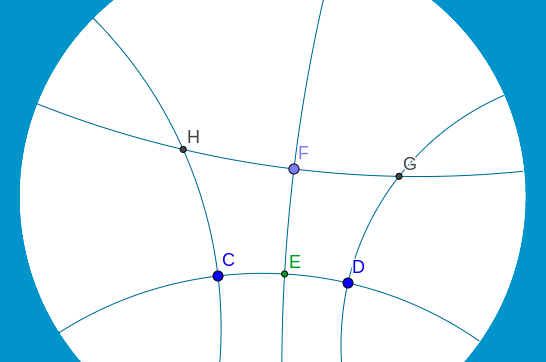
\includegraphics[width=\linewidth]{CartesianHyperbolicProblem.png}
		\caption{The Cartesian Hyperbolic Problem.}
		\label{fig:chp}
	\end{figure}
	
	It becomes intuitively obvious that the spatial density in the horizontal direction is something like $\cosh\pqty{y}$, but to prove it, we have this problem where
	$C=\pqty{0,0}, D=\pqty{0,\epsilon}, E=\pqty{0,\frac{\epsilon}{2}}, H=\pqty{0,y}, G=\pqty{\epsilon,y}$ and $F$ is the midpoint of $H$ and $G$.
	
	Noting $\angle{GDE}=\frac{\pi}{2}$, we have $\sin\pqty{\angle{DEG}}=\frac{\sinh\pqty{y}}{\sinh\pqty{\overline{EG}}}$,
	
	and $\tan\pqty{\angle{DEG}}=\frac{\tanh\pqty{y}}{\sinh\pqty{\frac{\epsilon}{2}}}$. Thus
	$$\overline{EG} = \arsinh\pqty{ \frac{\sinh\pqty{y}}{\sin\pqty{\arctan\pqty{\frac{\tanh\pqty{y}}{\sinh\pqty{\frac{\epsilon}{2}}}}}}}
	= \arsinh\pqty{
		\cosh\pqty{y}
		\sqrt{\sinh\pqty{\frac{\epsilon}{2}}^2+\tanh\pqty{y}^2}
	}$$
	
	Noting $\angle{EFG}=\frac{\pi}{2}$, we have $\sin\pqty{\angle{GEF}}=\frac{\sinh\pqty{\overline{FG}}}{\sinh\pqty{\overline{EG}}}$.
	
	Noting $\angle{DEG}+\angle{GEF}=\frac{\pi}{2}$, we have...
	$$\overline{FG} = \arsinh\pqty{
		\sin\pqty{\frac{\pi}{2}-\arctan\pqty{\frac{\tanh\pqty{y}}{\sinh\pqty{\frac{\epsilon}{2}}}}}
		\cosh\pqty{y}
		\sqrt{\sinh\pqty{\frac{\epsilon}{2}}^2+\tanh\pqty{y}^2}
	}$$
	Demanding $\epsilon>0$ allows further simplification:
	$$\overline{FG} = \arsinh\pqty{
		\cosh\pqty{y}
		\sqrt{\sinh\pqty{\frac{\epsilon}{2}}^2}
	} = \arsinh\pqty{
		\cosh\pqty{y}
		\sinh\pqty{\frac{\epsilon}{2}}
	}$$
	Now we can calculate the density of space in the horizontal direction!
	$$
	\lim\limits_{\epsilon\to 0^+}\frac{\overline{HG}}{\overline{CD}}=
	\lim\limits_{\epsilon\to 0^+}\frac{\overline{FG}}{\overline{ED}}=
	\lim\limits_{\epsilon\to 0^+}\frac{\arsinh\pqty{
			\cosh\pqty{y}
			\sinh\pqty{\frac{\epsilon}{2}}
	}}{\frac{\epsilon}{2}}
	=\cosh\pqty{y}
	$$
	
	Just as one might suspect, where $s$ is the length of a hyperbolic geodesic, the Cartesian Hyperbolic Plane Metric is:
	$$\pqty{ds}^2=\pqty{\cosh\pqty{y}*dx}^2+\pqty{1*dy}^2$$
	Alternately,
	$$\frac{ds}{dx}=\sqrt{\cosh\pqty{y}^2+\pqty{\frac{dy}{dx}}^2}$$
	
	\subsection{Cartesian Hyperbolic Plane Geodesics}
	Let $g\pqty{x}$ be a function of a geodesic. Then the length of a line segment is:
	$$\int_{a}^{b}\sqrt{\cosh\pqty{g\pqty{x}}^2+g'\pqty{x}^2}dx$$
	The Euler-Lagrange equations guarantee
	$$\frac{\cosh\pqty{g\pqty{x}}\sinh\pqty{g\pqty{x}}}{\sqrt{\cosh\pqty{g\pqty{x}}^2+g'\pqty{x}^2}}
	=\pdiff{x}{}\pqty{\frac{g'\pqty{x}}{\sqrt{\cosh\pqty{g\pqty{x}}^2+g'\pqty{x}^2}}}
	$$
	$$\frac{\cosh\pqty{g\pqty{x}}\sinh\pqty{g\pqty{x}}}{\sqrt{\cosh\pqty{g\pqty{x}}^2+g'\pqty{x}^2}}
	=\frac{\cosh\pqty{g\pqty{x}}\pqty{\cosh\pqty{g\pqty{x}}g''\pqty{x}-\sinh\pqty{g\pqty{x}}g'\pqty{x}^2}}
	{\pqty{\cosh\pqty{g\pqty{x}}^2+g'\pqty{x}^2}^{3/2}}
	$$
	$$\sinh\pqty{g\pqty{x}}\pqty{\cosh\pqty{g\pqty{x}}^2+g'\pqty{x}^2}
	=\cosh\pqty{g\pqty{x}}g''\pqty{x}-\sinh\pqty{g\pqty{x}}g'\pqty{x}^2
	$$
	$$\sinh\pqty{g\pqty{x}}\pqty{\cosh\pqty{g\pqty{x}}^2+2g'\pqty{x}^2}
	=\cosh\pqty{g\pqty{x}}g''\pqty{x}
	$$
	$$\tanh\pqty{g\pqty{x}}\pqty{\cosh\pqty{g\pqty{x}}^2+2g'\pqty{x}^2}=g''\pqty{x}$$
	
	All geodesics can be divided into 4 types of geodesics:
	
	The trivial cases $y=0$ and $x=c$ for $c\in\mathbb{R}$.
	
	Those that do not cross the x-axis.
	$$g_0(0)\in\mathbb{R}^+,g_0'(0)=0,g_0(x)=g_0(-x),y=\pm g_0(x-c_0),c_0\in\mathbb{R}$$
	$$g_0(x)=\artanh(\tanh(g_0(0))\cosh(x)),\abs{x}<\arcosh(\tanh(g_0(0))^{-1})$$
	
	Those that cross the x-axis. 
	$$g_1(0)=0,g_1'(0)\in\mathbb{R}^+,g_1(x)=-g_1(-x),y=\pm g_1(x-c_1),c_1\in\mathbb{R}$$
	$$g_1(x)=\artanh(g_1'(0)\sinh(x)),\abs{x}<\arsinh(g_1'(0)^{-1})$$
	
	Those that touch the x-axis once infinitely far from the origin.
	$$\lim_{x\to -\infty}g_2(x)=0,\lim_{h\to\infty}g_2(-1/h)=\infty,y=\pm g_2(\pm x-c_2),c_2\in\mathbb{R}$$
	$$g_2(x)=\artanh(\exp(x)),x<0$$
	
	All the geodesics $y=g\pqty{x}$ (the geodesics excluding $x=c$) can be written in the form
	$$g\pqty{x}\in\Bqty{\artanh(a_0\exp(x)+a_1\exp(-x))|\Bqty{a_0,a_1}\subset\mathbb{R}}$$
	
	This form makes it easy to verify that if we have 2 geodesics ($y=g_3\pqty{x}$ and $y=g_4\pqty{x}$) then we get the following geodesics free:
	$$\Bqty{\artanh(a_2\tanh\pqty{g_3\pqty{x}}+a_3\tanh\pqty{g_4\pqty{x}}|\Bqty{a_2,a_3}\subset\mathbb{R}}$$

	\subsection{Complex Cartesian Hyperbolic Plane Geodesics}
	If complex numbers are used instead of real numbers for $x$ and $y$, then new types of geodesics are discovered. Furthermore, there may be unknown complex geodesics.
	$$\Bqty{\artanh(a_0\exp(x)+a_1\exp(-x))|\Bqty{a_0,a_1}\subset\mathbb{C}}\subseteq\text{ComplexGeodesics}$$
	$$\Bqty{i\arcsin\pqty{\frac{\tanh\pqty{x-a_1}\sqrt{a_0-1}}{\sqrt{\tanh\pqty{x-a_1}^2a_0-1}}}|\Bqty{a_0,a_1}\subset\mathbb{C}}\subseteq\text{ComplexGeodesics}$$
	$$g\pqty{x}\in\text{ComplexGeodesics}\Leftrightarrow g\pqty{-x}\in\text{ComplexGeodesics}$$
	$$g\pqty{x}\in\text{ComplexGeodesics}\Leftrightarrow -g\pqty{x}\in\text{ComplexGeodesics}$$
	I conjecture that the following statement works because the analog worked with real numbers:
	$$\Bqty{g_3\pqty{x},g_4\pqty{x}}\subseteq\text{ComplexGeodesics}\Rightarrow$$
	$$\Bqty{\artanh(a_2\tanh\pqty{g_3\pqty{x}}+a_3\tanh\pqty{g_4\pqty{x}}|\Bqty{a_2,a_3}\subset\mathbb{C}}\subseteq\text{ComplexGeodesics}$$
\end{document}
